\documentclass{gescons}

\genre {Balanço}
%\author{Ricardo Rezende}
%\roles{Voluntário do Setor Comercial da Editares}
\title{Pontoações da Editares 21 Anos}



\begin{document}
    \makeentrevistatitle
    %\maketitle

    %\fullwidthimage{fields}{b}

    %\coverart{back/editorial}
    \coverart{../fundo-generico}
    % \vspace*{\fill}
    
    
\begin{center}
    
    %\includegraphics[height=5.8cm]{articles/balanco/grafico/balanco1} 
    %\includegraphics[height=5.8cm]{articles/balanco/grafico/balanco2}  
    %\includegraphics[height=5.8cm]{articles/balanco/grafico/balanco3}  
    %\includegraphics[height=7cm]{articles/balanco/grafico/balanco4}  
    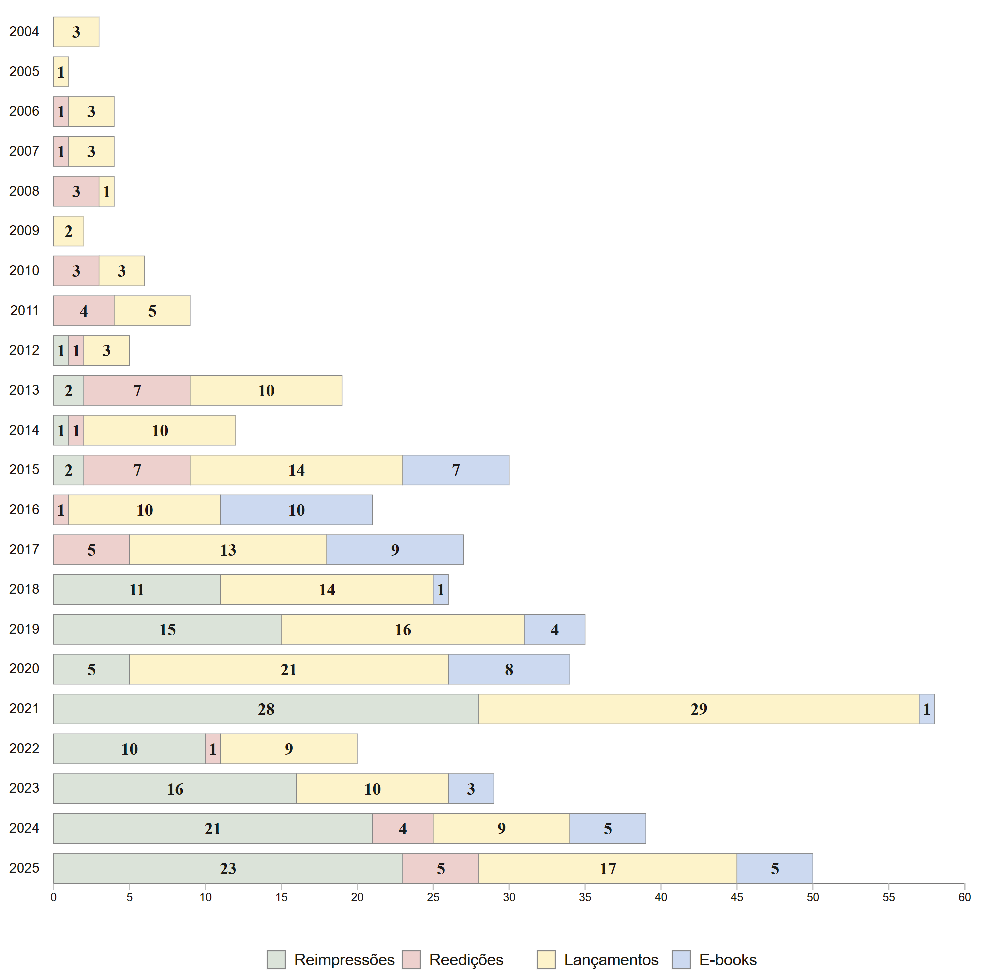
\includegraphics[width=\textwidth]{articles/balanco/grafico/grafico}  
\end{center}
    
%\begin{center}
%    \includegraphics[width=9cm]{articles/atualizacoes/fotos/escola-editores/escola-editores1.jpeg} 
%\end{center}

% \subsection*{Publicações da Editares 2004 a 2025}


\begin{longtable}[c]{|r|l|}
  \hline
  \multicolumn{2}{|c|}{\textbf{Total de Publicações da Editares (2004 a 2025)}} \\ \hline
  203 & Livros nacionais \\ \hline
  66 & Livros Traduzidos (Alemão, Árabe, Espanhol, Francês, Inglês, Italiano e Romeno) \\ \hline
  58 & E-books \\ \hline
  47 & Revistas \\ \hline
  178 & Autores \\ \hline
\end{longtable}



%    \end{multicols}
% \vspace*{\fill}
\end{document}
